%% talk1.tex
%% Copyright 2022 Tom M. Ragonneau
%
% This work may be distributed and/or modified under the
% conditions of the LaTeX Project Public License, either version 1.3
% of this license or (at your option) any later version.
% The latest version of this license is in
%   http://www.latex-project.org/lppl.txt
% and version 1.3 or later is part of all distributions of LaTeX
% version 2005/12/01 or later.
%
% This work has the LPPL maintenance status `maintained'.
%
% The Current Maintainer of this work is Tom M. Ragonneau.
\documentclass{polyu-presentation}
\usepackage[final]{microtype}

% List of hyphenation exceptions for US English
% Source: https://ctan.org/tex-archive/info/digests/tugboat/hyphenex
\input{ushyphex}

% Bibliographical resources
\addbibresource{ragonneau-bib/strings.bib}
\addbibresource{ragonneau-bib/optim.bib}

% Dedicated mathematical macros
\newcommand{\con}[1]{c_{#1}}
\newcommand{\ieq}{\mathcal{E}}
\newcommand{\iub}{\mathcal{I}}
\newcommand{\lag}{\mathcal{L}}
\newcommand{\obj}{f}

% Performance and data profiles
\usepackage{xstring}
\newcommand{\drawprofiles}[4]{%
    \def\selectsolvers{#2}%
    \def\selectcsv{figures/#3}%
    \def\selectprofile{#4}%
    \ifthenelse{\equal{#1}{performance}}{%
        \def\selectxlabel{$\log_2(\alpha)$}%
        \def\selectylabel{Performance profiles~$\rho_s(\alpha)$}%
    }{%
        \def\selectxlabel{Number of simplex gradients~$\alpha$}%
        \def\selectylabel{Data profiles~$d_s(\alpha)$}%
    }
    %% utils/profiles.tex
%% Copyright 2022 Tom M. Ragonneau
%
% This work may be distributed and/or modified under the
% conditions of the LaTeX Project Public License, either version 1.3
% of this license or (at your option) any later version.
% The latest version of this license is in
%   http://www.latex-project.org/lppl.txt
% and version 1.3 or later is part of all distributions of LaTeX
% version 2005/12/01 or later.
%
% This work has the LPPL maintenance status `maintained'.
%
% The Current Maintainer of this work is Tom M. Ragonneau.
\begin{tikzpicture}[scale=0.9]
    \pgfplotstableread[col sep=comma]{\selectcsv}\selectcsvread
    \newcommand{\getxmaxcsv}[1]{%
        \pgfplotstablegetrowsof{\selectcsvread}%
        \pgfmathtruncatemacro{\LastRowNo}{\pgfplotsretval-1}%
        \pgfplotstablesort[sort key={#1}]{\csvsorted}{\selectcsvread}%
        \pgfplotstablegetelem{\LastRowNo}{#1}\of{\csvsorted}%
        \pgfmathsetmacro{\selectxmaxcsv}{\pgfplotsretval}%
    }
    \pgfmathparse{\selectsolvers[0]}
    \let\selectsolver\pgfmathresult\relax
    \getxmaxcsv{x\selectprofile_\selectsolver}
    \begin{axis}[%
        width=205pt,%
        xmin=0,%
        xmax=0.55*\selectxmaxcsv,%
        ymin=0,%
        ymax=1,%
        minor y tick num=1,%
        yminorticks=true,%
        ytick={0,0.2,...,1},%
        cycle list name=profiles,%
        legend pos=south east,%
        xlabel={\selectxlabel},%
        ylabel={\selectylabel},%
        xticklabel style={/pgf/number format/1000 sep={}},%
    ]
        \pgfmathparse{dim{\selectsolvers}-1}
        \let\selectlastindex\pgfmathresult\relax
        \foreach \i in {0,1,...,\selectlastindex} {%
            \pgfmathparse{\selectsolvers[\i]}%
            \let\selectsolver\pgfmathresult\relax%
            \StrSubstitute{\selectsolver}{-}{~}[\selectsolverescaped]%
            \addplot table[%
            x=x\selectprofile_\selectsolver,%
            y=y\selectprofile,%
            col sep=comma,%
            ]{\selectcsvread};%
            \addlegendentryexpanded{\selectsolverescaped}%
        }
    \end{axis}
\end{tikzpicture}%
}
\newcommand{\drawperformanceprofiles}[3]{\drawprofiles{performance}{#1}{#2}{#3}}
\newcommand{\drawdataprofiles}[3]{\drawprofiles{data}{#1}{#2}{#3}}

\title{Model-Based DFO Methods and Software}
\subtitle{Talk no.\ 1 \textemdash\ Overview of DFO}
\author[Tom M. Ragonneau]{\texorpdfstring{
    Tom M. Ragonneau\\ 
    \footnotesize Co-supervised by Dr.\ Zaikun Zhang and by Prof.\ Xiaojun Chen
}{Tom M. Ragonneau}}
\institute[PolyU AMA]{
    Department of Applied Mathematics\\
    The Hong Kong Polytechnic University
}
\date{September 13, 2022 (Revised on September 19, 2022)}
\titlegraphic{}

\begin{document}

\begin{frame}
	\titlepage
\end{frame}

\begin{frame}
    \frametitle{Table of contents}
	\tableofcontents[hideallsubsections]
\end{frame}

\section{Introduction to DFO}

\begin{frame}
    \frametitle{What is DFO?}

    Derivative-free optimization (DFO) aims at minimizing a function~$\obj$ using only \alert{function values}.
    The function can be a \alert{blackbox}, resulting from \alert{experiments} or \alert{complex simulations} (PDE, \dots).

    \bigskip

    \begin{center}
        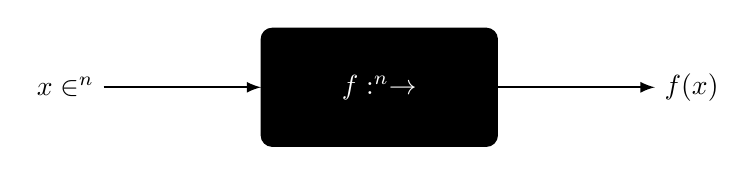
\begin{tikzpicture}
            \draw[thick,-latex] (0,0) -- (2,0);
            \draw[rounded corners,fill=black] (2,-0.75) rectangle (5,0.75);
            \draw[thick,-latex] (5,0) -- (7,0);
            \node[left] at (0,0) {$x \in \R^n$};
            \node at (3.5,0) {\textcolor{white}{$\obj : \R^n \to \R$}};
            \node[right] at (7,0) {$\obj(x)$};
        \end{tikzpicture}
    \end{center}

    \bigskip

    \begin{block}{}
        \begin{enumerate}
            \item $\obj$ may be smooth, but derivatives \alert{cannot be evaluated}.
            \item Each objective function evaluation is \alert{expensive}.
            \item The complexity measure is the \alert{number of function evaluations}.
        \end{enumerate}
    \end{block}
\end{frame}

\begin{frame}
    \frametitle{Fairy tale vs.\ reality}

    \alert<2>{The reality} is often more complex than \alert<1>{the theory}.

    \bigskip
    
    \begin{center}
        \begin{tikzpicture}
            \begin{axis}[%
                colormap/viridis,%
                xmin=-5,%
                xmax=5,%
                ymin=-5,%
                ymax=5,%
                zmin=-5,%
                zmax=55,%
                xlabel={$x_1$},%
                ylabel={$x_2$},%
                zlabel={$\obj(x)$},%
            ]
                \only<1>{
                    \addplot3[%
                        domain=-5:5,%
                        domain y=-5:5,%
                        samples=60,%
                        surf,%
                    ]{x^2+sin(250*x)+y^2+sin(250*y)};
                }
                \only<2>{
                    \addplot3[%
                        domain=-5:5,%
                        domain y=-5:5,%
                        samples=60,%
                        surf,%
                    ]{x^2+sin(250*x)+y^2+sin(250*y)+rand};
                }
            \end{axis}
        \end{tikzpicture}
    \end{center}
\end{frame}

\begin{frame}
    \frametitle{Mathematical formulation}

    The problem is
    \begin{align*}
        \min_{x \in \R^n}   & \quad \obj(x)\\
        \text{s.t.}         & \quad \con{i}(x) \le 0, ~ i \in \iub,\\
                            & \quad \con{i}(x) = 0, ~ i \in \ieq,
    \end{align*}
    where~$\obj : \R^n \to \R$ is the \alert{objective function} and~$\con{i} : \R^n \to \R$ are the \alert{constraint functions}.

    \smallskip

    \begin{block}{}
        \begin{enumerate}
            \item The \alert{feasible set} is
            \begin{equation*}
                \Omega = \set{x \in \R^n : \con{i}(x) \le 0, ~ i \in \iub ~ \mathrm{and} ~ \con{i}(x) = 0, ~ i \in \ieq}.
            \end{equation*}
            \item The derivatives of~$\obj$ and~$\con{i}$ are \alert{unknown}.
            \item \alert{No structure} of the problem (e.g., convexity) is assumed.
        \end{enumerate}
    \end{block}
\end{frame}

\section{Examples of applications}

\begin{frame}
    \frametitle{Examples of DFO problems I}

    \begin{block}{Stability of the Gaussian elimination~\parencite{Higham_1993}}
        We can measure the \alert{stability} of the \alert{Gaussian elimination} by
        \begin{equation*}
            \max_{A \in \R^{n \times n}} \rho_n(A),
        \end{equation*}
        where~$\rho_n(A)$ is the \alert{growth factor} of~$A$, given by
        \begin{equation*}
            \rho_n(A) = \frac{1}{\norm{A}_{\max}} \max_{0 \le k \le n - 1} \norm{A^{(k)}}_{\max},
        \end{equation*}
        with~$A^{(k)}$ being the~$k$th matrix of the Gaussian elimination.

        \begin{enumerate}
            \item Insights about the \alert{worst-case scenario}.
            \item Starting point for \alert{theoretical analyses}.
        \end{enumerate}
    \end{block}

    \medskip

    What is~\alert{$\nabla \rho_n$}? Does it even exist?
\end{frame}

\begin{frame}
    \frametitle{Examples of DFO problems II}

	\begin{figure}
		\centering
		\begin{tikzpicture}
			\uncover<2>{
				\draw[pattern=north east lines,pattern color=DarkOrchid!25,rounded corners] (8,3) rectangle (11,4.5);
			}
			\draw[thick,rounded corners] (0,0) rectangle (3,1.5);
			\draw[thick,rounded corners] (0,4) rectangle (3,5.5);
			\draw[thick,rounded corners] (4,2) rectangle (7,3.5);
			\draw[thick,rounded corners] (8,1) rectangle (11,2.5);
			\draw[thick,rounded corners] (8,3) rectangle (11,4.5);
			\draw[thick,-latex] (3,1) -- (5.5,1) -- (5.5,2);
			\draw[thick] (3,0.5) -- (7.5,0.5) -- (7.5,2.5) -- (7,2.5);
			\draw[thick,-latex] (7.5,1.75) -- (8,1.75);
			\draw[thick] (3,4.75) -- (7.5,4.75) -- (7.5,3) -- (7,3);
			\draw[thick,-latex] (7.5,3.75) -- (8,3.75);
			\node at (0.6,0.75) {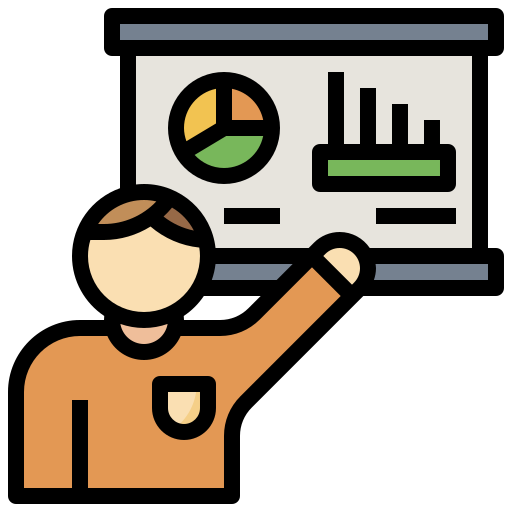
\includegraphics[height=0.8cm]{images/machine-learning/presentation.png}};
			\node at (0.6,4.75) {
\includegraphics[height=0.8cm]{images/machine-learning/checklist.png}};
			\node at (4.6,2.75) {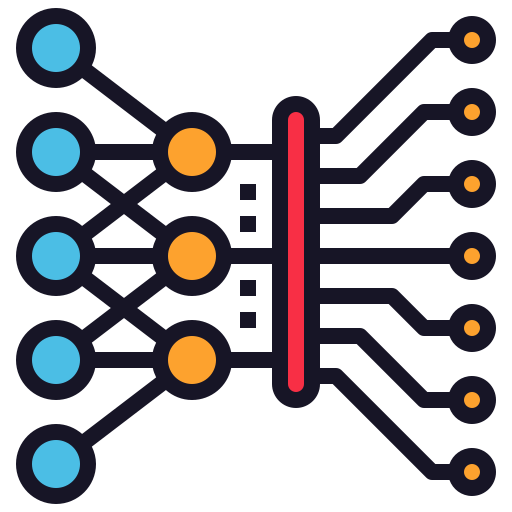
\includegraphics[height=0.8cm]{images/machine-learning/deep-learning.png}};
			\node at (8.6,1.75) {
\includegraphics[height=0.8cm]{images/machine-learning/good.png}};
			\node at (8.6,3.75) {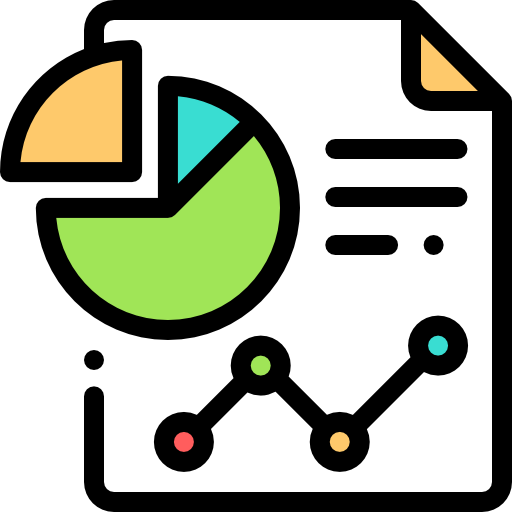
\includegraphics[height=0.8cm]{images/machine-learning/result.png}};
			\node at (2,0.75) {\makecell{Training\\ dataset}};
			\node at (2,4.75) {\makecell{Testing\\ dataset}};
			\node at (6,2.75) {\makecell{Machine\\ learning}};
			\node at (10,1.75) {\makecell{Training\\ accuracy}};
			\node at (10,3.75) {\makecell{Testing\\ accuracy}};
			\uncover<2>{
				\draw[pattern=north east lines,pattern color=DarkOrchid!25,rounded corners] (0,2) rectangle (3,3.5);
				\draw[thick,rounded corners] (0,2) rectangle (3,3.5);
				\draw[thick,-latex] (3,2.75) -- (4,2.75);
				\node at (0.6,2.75) {
\includegraphics[height=0.8cm]{images/machine-learning/technical-support.png}};
				\node at (2,2.75) {\makecell{Hyperpa-\\ rameters}};
			}
		\end{tikzpicture}
	\end{figure}

	\smallskip

	\uncover<2>{
		\begin{block}{}
            \begin{enumerate}
                \item How to \alert{maximize} the testing accuracy by tuning the \alert{hyperparameters}?
                \item What is the gradient of the testing accuracy?
            \end{enumerate}
		\end{block}
	}
\end{frame}

\section{Optimality conditions for smooth optimization}

\begin{frame}
    \frametitle{What is a solution?}

    \begin{block}{}
        A point~$x^{\ast} \in \Omega$ is
        \begin{enumerate}
            \item a \textcolor{OliveGreen}{global solution} if~$\obj(x) \ge \obj(x^{\ast})$ for all~$x \in \Omega$, and
            \item a \textcolor{BurntOrange}{local solution} if there exists a neighborhood~$\mathcal{N} \subseteq \R^n$ of~$x^{\ast}$ such that~$\obj(x) \ge \obj(x^{\ast})$ for all~$x \in \mathcal{N} \cap \Omega$.
        \end{enumerate}
    \end{block}

    \smallskip

    \begin{center}
        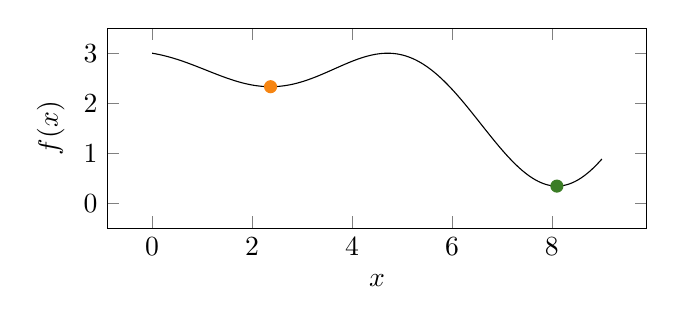
\begin{tikzpicture}
            \begin{axis}[%
                axis equal image,
                ymin=-0.5,
                ymax=3.5,
                xlabel={$x$},%
                ylabel={$f(x)$},%
            ]
                \addplot[domain=0:9,samples=200,smooth] {-x*(sin(360*x/(2*pi))+1)/6+3};
                \draw[color=BurntOrange,fill=BurntOrange] (2.3695,2.32958) circle (0.12);
                \draw[color=OliveGreen,fill=OliveGreen] (8.09966,0.340649) circle (0.12);
            \end{axis}
        \end{tikzpicture}
    \end{center}

    We \alert{do not seek} local or global solutions! They are \alert{too difficult} to find.
\end{frame}

\begin{frame}
    \frametitle{First-order optimality conditions}

    Let~$\lag$ be the \alert{Lagrangian function}, i.e.,
    \begin{equation*}
        \lag(x, \lambda) = f(x) + \sum_{\mathclap{i \in \iub \cup \ieq}} \lambda_i \con{i}(x), \quad \text{for~$x \in \R^n$ and~$\lambda_i \in \R$.}
    \end{equation*}

    \begin{block}{First-order necessary conditions (KKT conditions)}
        Let~$x^{\ast}$ be a \alert{local solution}.
        Under standard assumptions, there exists a \alert{Lagrange multiplier}~$\lambda^{\ast}$ such that
        \begin{empheq}[left=\empheqlbrace]{alignat*=1}
            & \nabla_x \lag(x^{\ast}, \lambda^{\ast}) = 0,\\
            & \con{i}(x^{\ast}) \le 0, ~ i \in \iub,\\
            & \con{i}(x^{\ast}) = 0, ~ i \in \ieq,\\
            & \lambda_i^{\ast} \con{i}(x^{\ast}) = 0, ~ i \in \iub,\\
            & \lambda_i^{\ast} \ge 0, ~ i \in \iub.
        \end{empheq}
    \end{block}
\end{frame}

\begin{frame}
    \frametitle{Second-order optimality conditions}

    Let~$\mathcal{A}(x)$ be the \alert{active set} at~$x$, i.e.,
    \begin{equation*}
        \mathcal{A}(x) = \ieq \cup \set{i \in \iub : \con{i}(x) \ge 0}.
    \end{equation*}

    \begin{block}{Second-order necessary conditions}
        Let~$x^{\ast}$ be a \alert{local solution}.
        Given a \alert{Lagrange multiplier}~$\lambda^{\ast}$ satisfying the KKT conditions, let~$z \in \R^n$ be any vector such that
        \begin{subequations}
            \label{eq:second-order}
            \begin{empheq}[left=\empheqlbrace]{alignat=1}
                & \nabla \con{i}(x^{\ast})^{\T} z = 0, ~ i \in \ieq,\\
                & \nabla \con{i}(x^{\ast})^{\T} z = 0, ~ i \in \mathcal{A}(x^{\ast}) \cap \iub, ~ \lambda_i^{\ast} > 0,\\
                & \nabla \con{i}(x^{\ast})^{\T} z \ge 0, ~ i \in \mathcal{A}(x^{\ast}) \cap \iub, ~ \lambda_i^{\ast} = 0.
            \end{empheq}
        \end{subequations}
        Then~$z^{\T} \nabla_{x, x}^2 \lag(x^{\ast}, \lambda^{\ast}) z \ge 0$.
    \end{block}

    If~$z^{\T} \nabla_{x, x}^2 \lag(x^{\ast}, \lambda^{\ast}) z > 0$ for all~$z$, the conditions are \alert{sufficient}.
\end{frame}

\section{Trust-region methods}

\begin{frame}
    \frametitle{Methodology of DFO}

    \alert{Two main strategies} underlies the DFO methods.
    \begin{enumerate}
        \item \alert{Direct-search} methods select iterates only using simple comparisons.
        They are easy to implement but slow in practice.
        \item \alert{Model-based} methods select iterates according to models of~$\obj$ and~$\Omega$.
        They are hard to implement but fast in practice.
        \begin{enumerate}
            \item \alert{Line-search} methods: they perform a one-dimensional searches along directions provided by the models.
            \item \alert{Trust-region} methods: our interest.
            For simplicity, here~$\Omega = \R^n$.
            Given~$m^k$ a model of~$\obj$ around~$x^k$, let
            \begin{equation*}
                d^k \approx \argmin_{d \in \R^n} \set{m^k(x^k + d) : \norm{d} \le \Delta^k}
            \end{equation*}
            for some~$\Delta^k$.
            Then
            \begin{empheq}[left={x^{k + 1} = \empheqlbrace}]{alignat*=2}
                & x^k + d^k   && \quad \text{if sufficient decrease of~$\obj$,}\\
                & x^k         && \quad \text{otherwise.}
            \end{empheq}
        \end{enumerate}
    \end{enumerate}
\end{frame}

\begin{frame}
    \frametitle{Trust-region methods in unconstrained optimization}

    \foreach \n in {1,...,19}{
        \only<\n>{
            \begin{center}
                \includegraphics[width=.9\textwidth]{images/trust-region/tr\n.pdf}
            \end{center}
        }
    }
\end{frame}

\begin{frame}
    \frametitle{Assessing the performance of the models}

    The problem is
	\begin{equation*}
        \min_{x \in \R^n} \obj(x).
    \end{equation*}

	\begin{block}{How to assess the performance of the model?}
		Let~$m^k$ be the~$k$th \alert{model}.
        Define the \alert{trust-region ratio}
		\begin{equation*}
            \rho^k = \frac{f(x^k) - f(x^k + d^k)}{m^k(x^k) - m^k(x^k + d^k)}.
        \end{equation*}
		Let~$\Delta^k$ be the current trust-region radius.

		\begin{center}
			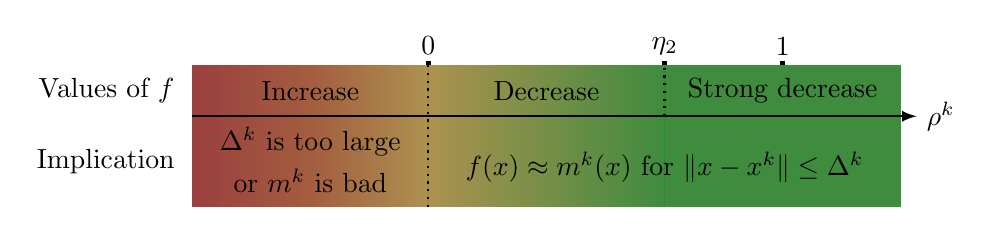
\begin{tikzpicture}
				\fill [left color=BrickRed,right color=Goldenrod,opacity=0.5] (-3,-1.15) rectangle (0,0.65);
				\fill [left color=Goldenrod,right color=OliveGreen,opacity=0.5] (0,-1.15) rectangle (3,0.65);
				\fill [left color=OliveGreen,right color=OliveGreen,opacity=0.5] (3,-1.15) rectangle (6,0.65);

				\draw [thick,-latex] (-3,0) -- (6.2,0) node [right] {$\rho^k$};
				\draw [thick,dotted] (0,-1.15) -- (0,0.65) node [above] {$0$};
				\draw [thick,dotted] (3,0) -- (3,0.65) node [above] {$\eta_2$};
				\draw [ultra thick] (0,0.65) -- (0,0.7);
				\draw [ultra thick] (3,0.65) -- (3,0.7);
				\draw [ultra thick] (4.5,0.65) -- (4.5,0.7);
				\node [above] at (4.5,0.65) {$1$};

				\node [left] at (-3.1,0.325) {Values of~$\obj$};
				\node [left] at (-3.1,-0.575) {Implication};
				\node at (-1.5,0.325) {Increase};
				\node at (-1.5,-0.325) {$\Delta^k$ is too large};
				\node at (-1.5,-0.825) {or~$m^k$ is bad};
				\node at (1.5,0.325) {Decrease};
				\node at (3,-0.65) {$\obj(x) \approx m^k(x)$  for~$\|x - x^k\| \leq \Delta^k$};
				\node at (4.5,0.325) {Strong decrease};
			\end{tikzpicture}
		\end{center}
	\end{block}
\end{frame}

% \begin{frame}{Unconstrained trust-region framework}
% 	\begin{algorithm}[H]
% 		\DontPrintSemicolon
% 		\KwData{Objective function~$\obj$, current iterate~$x^k$, current trust-region radius~$\Delta^k$, and constants~$0 \le \eta_0 \le \eta_1 \le \eta_2 < 1$ and~$0 \le \theta_1 < 1 < \theta_2$.}
%         Define~$m^k$ and calculate~$d^k$ by solving approximately
%         \vspace{-0.4\baselineskip}\begin{algomathdisplay}
%             \min_{d \in \R^n} \obj(x^k + d) \quad \text{s.t.} \quad \norm{d} \le \Delta^k
%         \end{algomathdisplay}\vspace{-0.4\baselineskip}
%         Evaluate the trust-region ratio~$\rho^k$\;
% 		\eIf{$\rho^k \ge \eta_0$}{
% 			Update the trial point~$x^{k + 1} \gets x^k + d^k$\;
% 		}{
% 			Retain the trial point~$x^{k + 1} \gets x^k$\;
% 		}
%         Update the trust-region radius
%         \vspace{-0.4\baselineskip}\begin{algoempheq}[left={\Delta^{k + 1} \gets \empheqlbrace}]{alignat*=2}
%             & \theta_1 \Delta^k && \quad \text{if~$\rho^k \le \eta_1$,}\\
%             & \Delta^k          && \quad \text{if~$\eta_1 < \rho^k \le \eta_2$,}\\
%             & \theta_2 \Delta^k && \quad \text{otherwise.}
%         \end{algoempheq}\vspace{-0.4\baselineskip}
% 		\caption{The~$k$th iteration of a trust-region method}
% 	\end{algorithm}
% \end{frame}

\section{Benchmarking tools for DFO methods}

\begin{frame}
    \frametitle{Description of the experiments}

    We compare the three unconstrained DFO solvers
    \begin{enumerate}
        \item \alert{NEWUOA}~\parencite{Powell_2006,Powell_2008},
        \item \alert{BFGS} with forward finite difference, and
        \item \alert{CG} with forward finite difference.
    \end{enumerate}

    \medskip

    We compare them on unconstrained problems that are
    \begin{enumerate}
        \item from the \alert{CUTEst} dataset~\parencite{Gould_Orban_Toint_2015}, and
        \item of dimension at most \num{50}.
    \end{enumerate}

    \medskip

    We employ the Python libraries
    \begin{enumerate}
        \item \alert{PDFO}, which provides NEWUOA;
        \item \alert{SciPy}, which provides BFGS and CG; and
        \item \alert{PyCUTEst}, which provides the CUTEst problems.
    \end{enumerate}
\end{frame}

\begin{frame}
    \frametitle{Description of the experiments}

    The problems are
    \begin{enumerate}
        \item \alert{unmodified} in the first experiment; and
        \item \alert{noisy} in the second experiment (relative noise), replacing~$f$ with
        \begin{equation*}
            \tilde{\obj}(x) = [1 + \epsilon(x)] \obj(x),
        \end{equation*}
        where~$\epsilon(x) \sim N(0, \sigma^2)$, for some~$\sigma > 0$.
    \end{enumerate}

    \bigskip

    We use \alert{performance and data profiles}~\parencite{Dolan_More_2002}.
    
    The \alert{convergence test} for DFO~\parencite{More_Wild_2009} is
    \begin{equation*}
        \obj(x^k) \le \obj_{\min} + \tau [\obj(x^0) - \obj_{\min}],
    \end{equation*}
    for some~$\tau > 0$, where~$\obj_{\min}$ is the least function value achieved by all solvers.
\end{frame}

\begin{frame}
    \frametitle{First experiment}

    We compare the solvers
    \begin{enumerate}
        \item on \alert{unmodified} problems,
        \item with~$\tau = 10^{-3}$, and
        \item using \alert{\only<1>{performance}\only<2>{data} profiles}.
    \end{enumerate}

    \only<1>{
        \begin{center}
            \drawperformanceprofiles{{"NEWUOA","BFGS","CG"}}{plain-1-50-perf-bfgs-cg-newuoa-u.csv}{3}
        \end{center}
    }
    \only<2>{
        \begin{center}
            \drawdataprofiles{{"NEWUOA","BFGS","CG"}}{plain-1-50-data-bfgs-cg-newuoa-u.csv}{3}
        \end{center}
    }
\end{frame}

\begin{frame}
    \frametitle{Second experiment}

    We compare the solvers
    \begin{enumerate}
        \item on \alert{noisy} problems with~$\sigma = 10^{-\only<1,4>{10}\only<2,5>{8}\only<3,6>{6}}$,
        \item with~$\tau = 10^{-3}$, and
        \item using \alert{\only<1,2,3>{performance}\only<4,5,6>{data} profiles}.
    \end{enumerate}

    \only<1>{
        \begin{center}
            \drawperformanceprofiles{{"NEWUOA","BFGS","CG"}}{noisy-1-50-10-perf-bfgs-cg-newuoa-u.csv}{3}
        \end{center}
    }
    \only<2>{
        \begin{center}
            \drawperformanceprofiles{{"NEWUOA","BFGS","CG"}}{noisy-1-50-8-perf-bfgs-cg-newuoa-u.csv}{3}
        \end{center}
    }
    \only<3>{
        \begin{center}
            \drawperformanceprofiles{{"NEWUOA","BFGS","CG"}}{noisy-1-50-6-perf-bfgs-cg-newuoa-u.csv}{3}
        \end{center}
    }
    \only<4>{
        \begin{center}
            \drawdataprofiles{{"NEWUOA","BFGS","CG"}}{noisy-1-50-10-data-bfgs-cg-newuoa-u.csv}{3}
        \end{center}
    }
    \only<5>{
        \begin{center}
            \drawdataprofiles{{"NEWUOA","BFGS","CG"}}{noisy-1-50-8-data-bfgs-cg-newuoa-u.csv}{3}
        \end{center}
    }
    \only<6>{
        \begin{center}
            \drawdataprofiles{{"NEWUOA","BFGS","CG"}}{noisy-1-50-6-data-bfgs-cg-newuoa-u.csv}{3}
        \end{center}
    }
\end{frame}

\section{Conclusion}

\begin{frame}
    \frametitle{Conclusion}
    
    In this talk, we presented
    \begin{enumerate}
        \item several \alert{concepts of DFO} and two examples of \alert{applications};
        \item the \alert{optimality conditions} for smooth optimization;
        \item the \alert{trust-region methods} for unconstrained optimization; and
        \item a few \alert{performance and data profiles} for DFO.
    \end{enumerate}

    \bigskip

    In the next talk, we will discuss \alert{interpolation models for DFO}.
\end{frame}

\appendix

\begin{frame}[t,allowframebreaks]
    \frametitle{References}

	\printbibliography
\end{frame}

\end{document}